%\vspace{10pt}
\section{Nonlinearity and Write Current Scaling}\label{sec:scale}
%\section{Nonlinearity and Write Current Scaling}\label{sec:scale}
%\subsection{Nonlinearity of the ReRAM Cell.} \vspace{6pt}
\begin{figure}[!b]
\centering
  % Requires \usepackage{graphicx}
  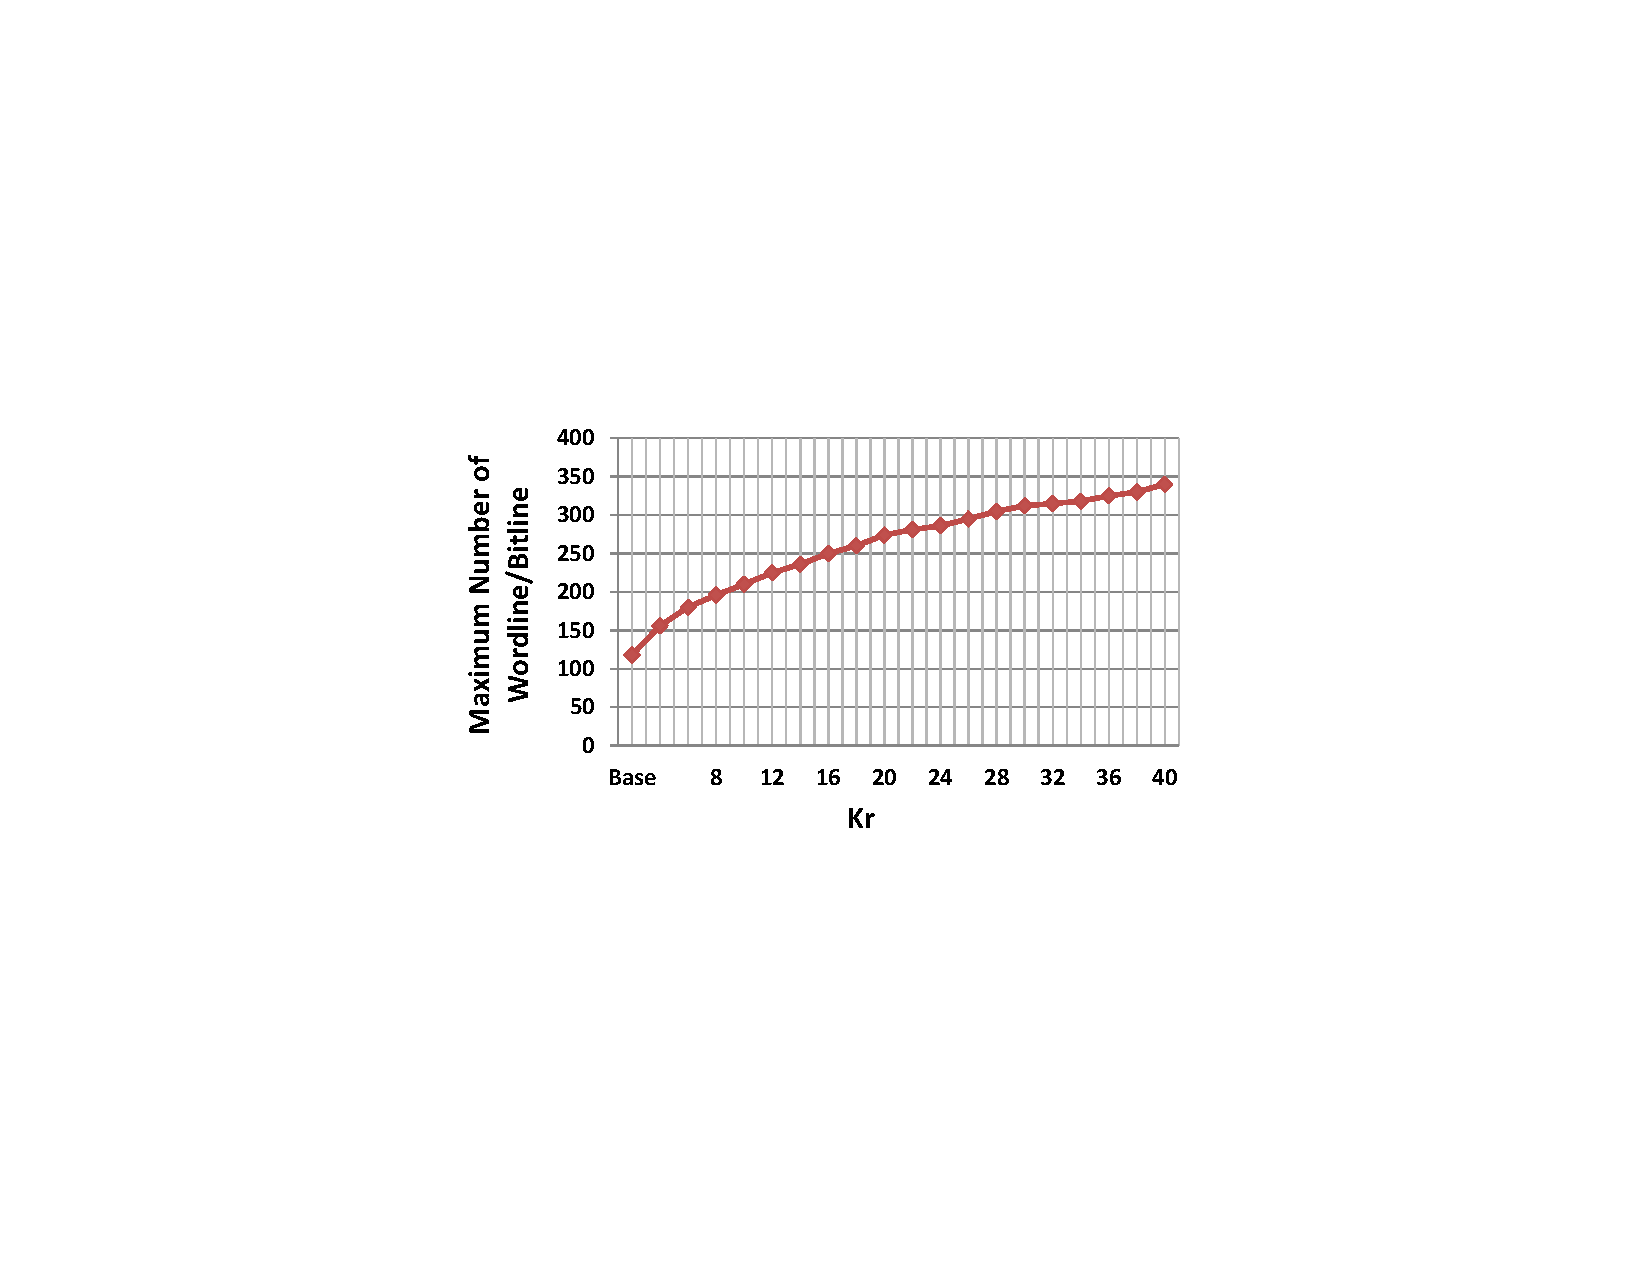
\includegraphics[width=0.45\textwidth]{./figures/non_linear_f}\\
  \vspace{-5pt}
  \caption{The maximum array size with different nonlinearity coefficients.}\label{fig:non_linear}
\end{figure}
One of the most distinct features of ReRAM is its nonlinearity. Normally,
the $K_r(p,V)$ value for memristor-based ReRAM is larger than 20, meaning
that the resistance of a half-biased cell is at least 10 times larger than
a full-biased cell. Clearly, the ReRAM cell with a larger nonlinearity
coefficient results in a better memory cell since the sneak current in
half selected cells will be significantly reduced. In addition, the
increased resistance at half-selected and unselected cells can also
mitigate the voltage drop along the activated wordline and bitline.
Besides, we find that the cross-point array design can also benefit from
the scaling of the write current. Figure~\ref{fig:non_linear} shows the
influence of different nonlinearity coefficients and write current on the
array size requirements for single-bit HWHB writing scheme. This figure
shows that the array size limitation is relaxed as the nonlinearity
increases or the write current scales. As we can tell from the figure, the
maximum array size exceeds $1024\times 1024$ when we have a nonlinearity
of $30$ together with a write current of $40\mu A$.

Moreover, the increase of nonlinearity or scaling of write current can
also reduce the energy consumption and area overhead of the cross-point
array. As shown in Figure~\ref{fig:E_and_A}(a), for a $512 \times 512$
array, the energy consumption for the write operation decreases
dramatically with the scaling of nonlinearity coefficient $K_r$. For
example, for a ReRAM cell with write current of 50uA, the write energy is
reduced by 98.3\% when $K_r$ decreases from 1 to 40. The area overhead of
the voltage drivers is illustrated in Figure~\ref{fig:E_and_A}(b). As a
baseline design ($K_r=20$ and $I_w=40\mu A$), the driver area overhead is
about 35\% the area of the memory array cells. To design a memory array
with effective cell size close to $4F^2$, we need to make sure the
nonlinearity and write current should satisfy certain conditions that the
driver overhead is less than 100\% so that the wordline drivers can be
almost "hidden" underneath the ReRAM cells. As nonlinearity and write
current continues to scale, the area overhead can be as low as 10\%. In
that case, the introduction of 3D stacking of multi-layer cross-point
arrays is meaningful in further reducing the effective cell size to $4/N_l
F^2$ where $N_l$ is the number of layers.

%Therefore, we can conclude that, the ReRAM cells with a small nonlinearity coefficient are not suitable for the cross-point structure based memory array. Next, we study the area overhead of multi-bit write. Figure~\ref{fig:Area_kr20} shows the normalized areas of the voltage drivers for one bit and multi-bit write operations. As mentioned, multi-bit write operations require larger driven current. Therefore, the area of voltage drivers for multi-bit write operations are much larger than that for one bit write operations. Finally, normalized areas of the one bit and multi-bit write operations have opposite trends as the array size increases. Normalized area for one bit write operation increases with the array size. On the contrary, normalized area for multi-bit write decreases as the array size increase.}

%\begin{figure}%[!t]
%\centering
%  % Requires \usepackage{graphicx}
%  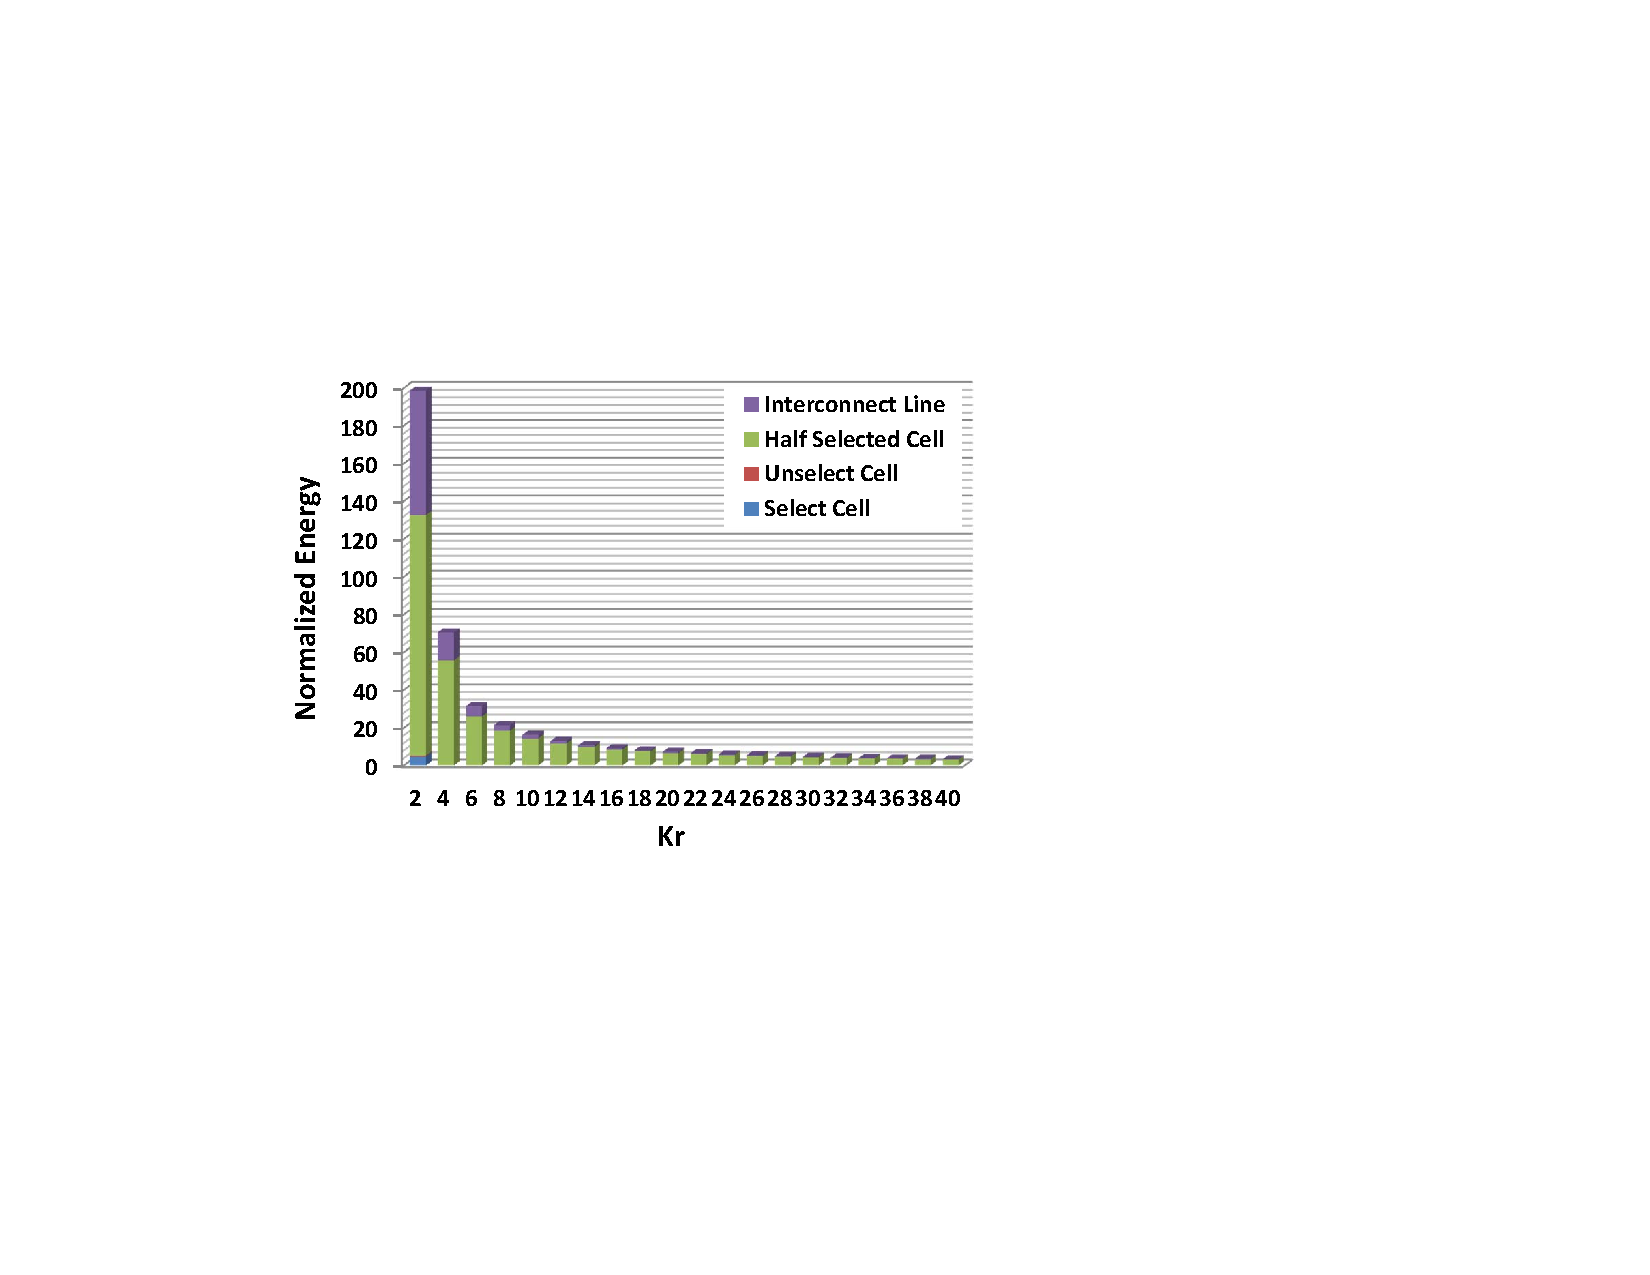
\includegraphics[width=0.38\textwidth]{./figures/non_linear_energy.pdf}\\
%  \caption{The normalized energy consumption with nonlinear ReRAM cells.}\label{fig:non_linear_energy}
%\end{figure}

%\begin{figure}%[!t]
%\centering
%  % Requires \usepackage{graphicx}
%  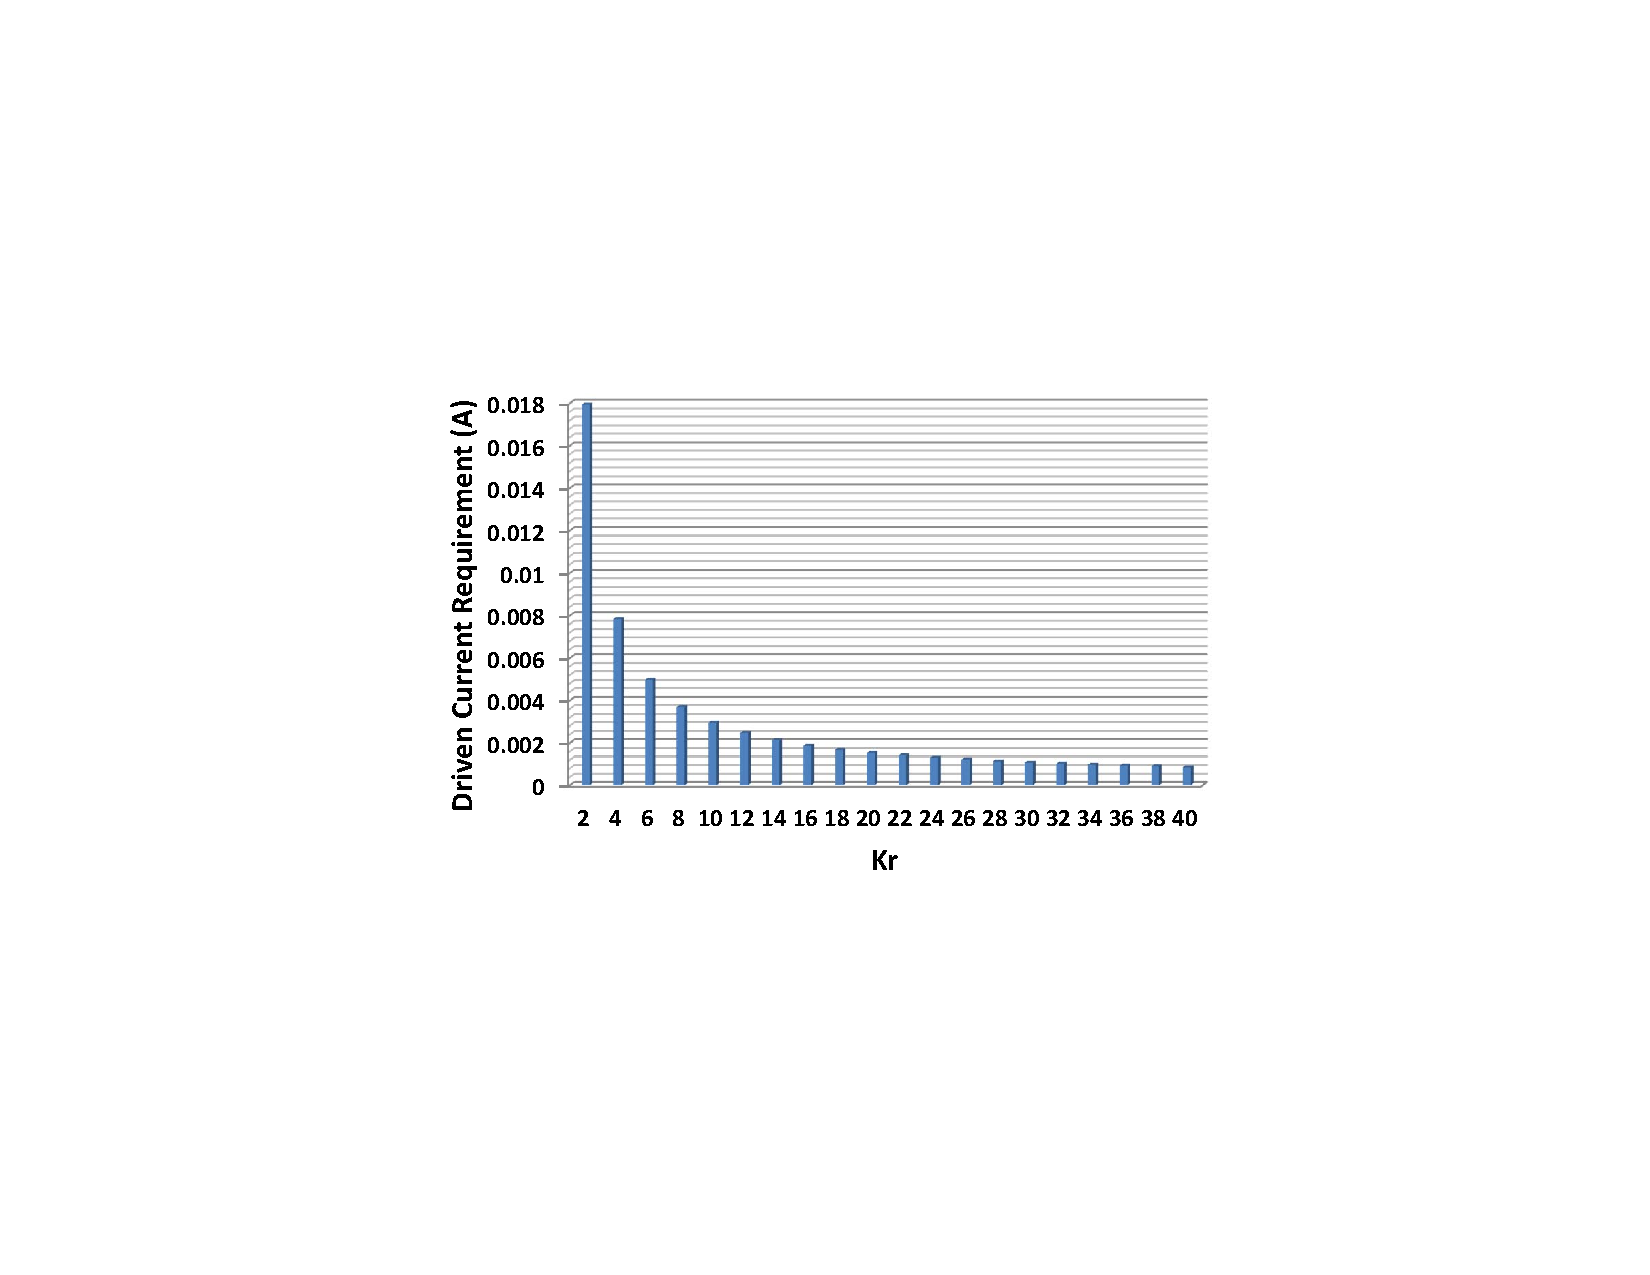
\includegraphics[width=0.4\textwidth]{./figures/non_linear_I.pdf}\\
%  \caption{The}\label{fig:non_linear_I}
%\end{figure}
%
%\begin{figure}%[!t]
%\centering
%  % Requires \usepackage{graphicx}
%  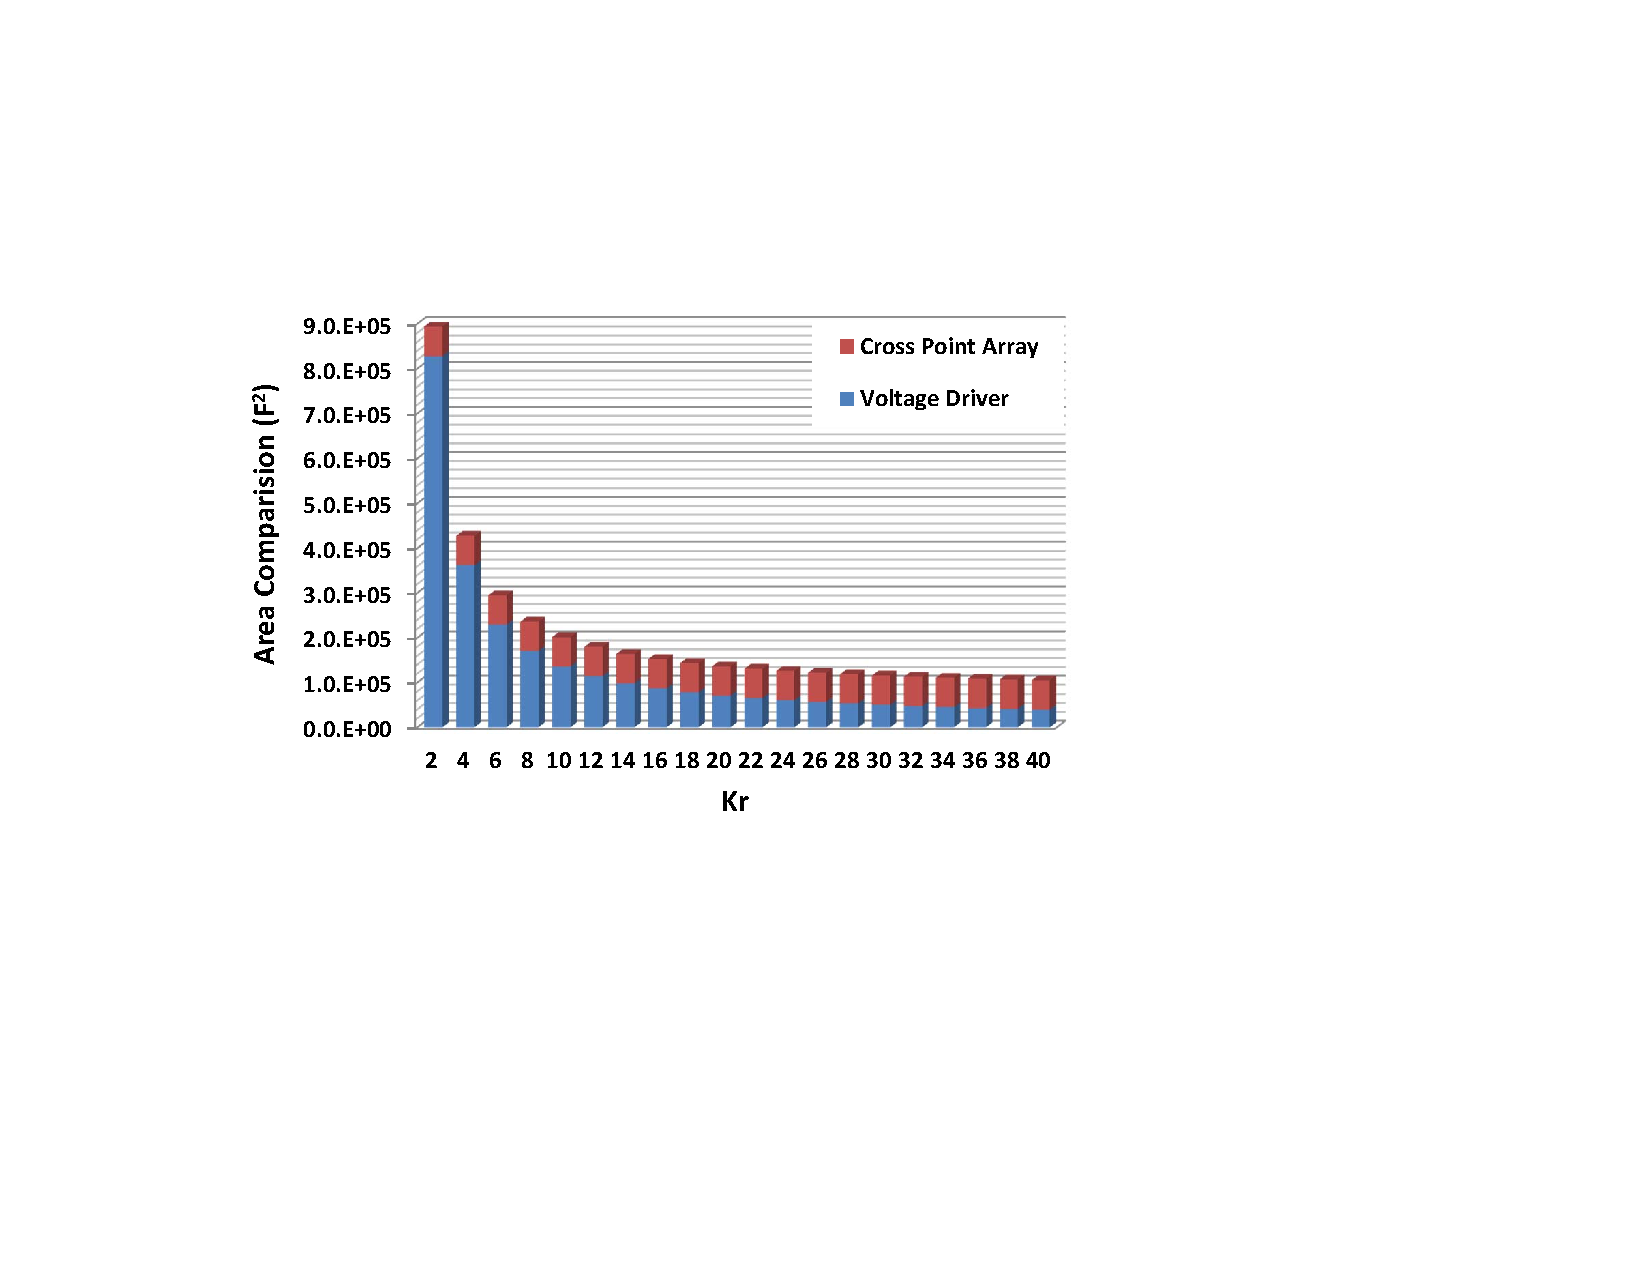
\includegraphics[width=0.4\textwidth]{./figures/non_linear_ara.pdf}\\
%  \caption{The}\label{fig:non_linear_ara}
%\end{figure}
%\begin{figure}%[!t]
%\centering
%  % Requires \usepackage{graphicx}
%  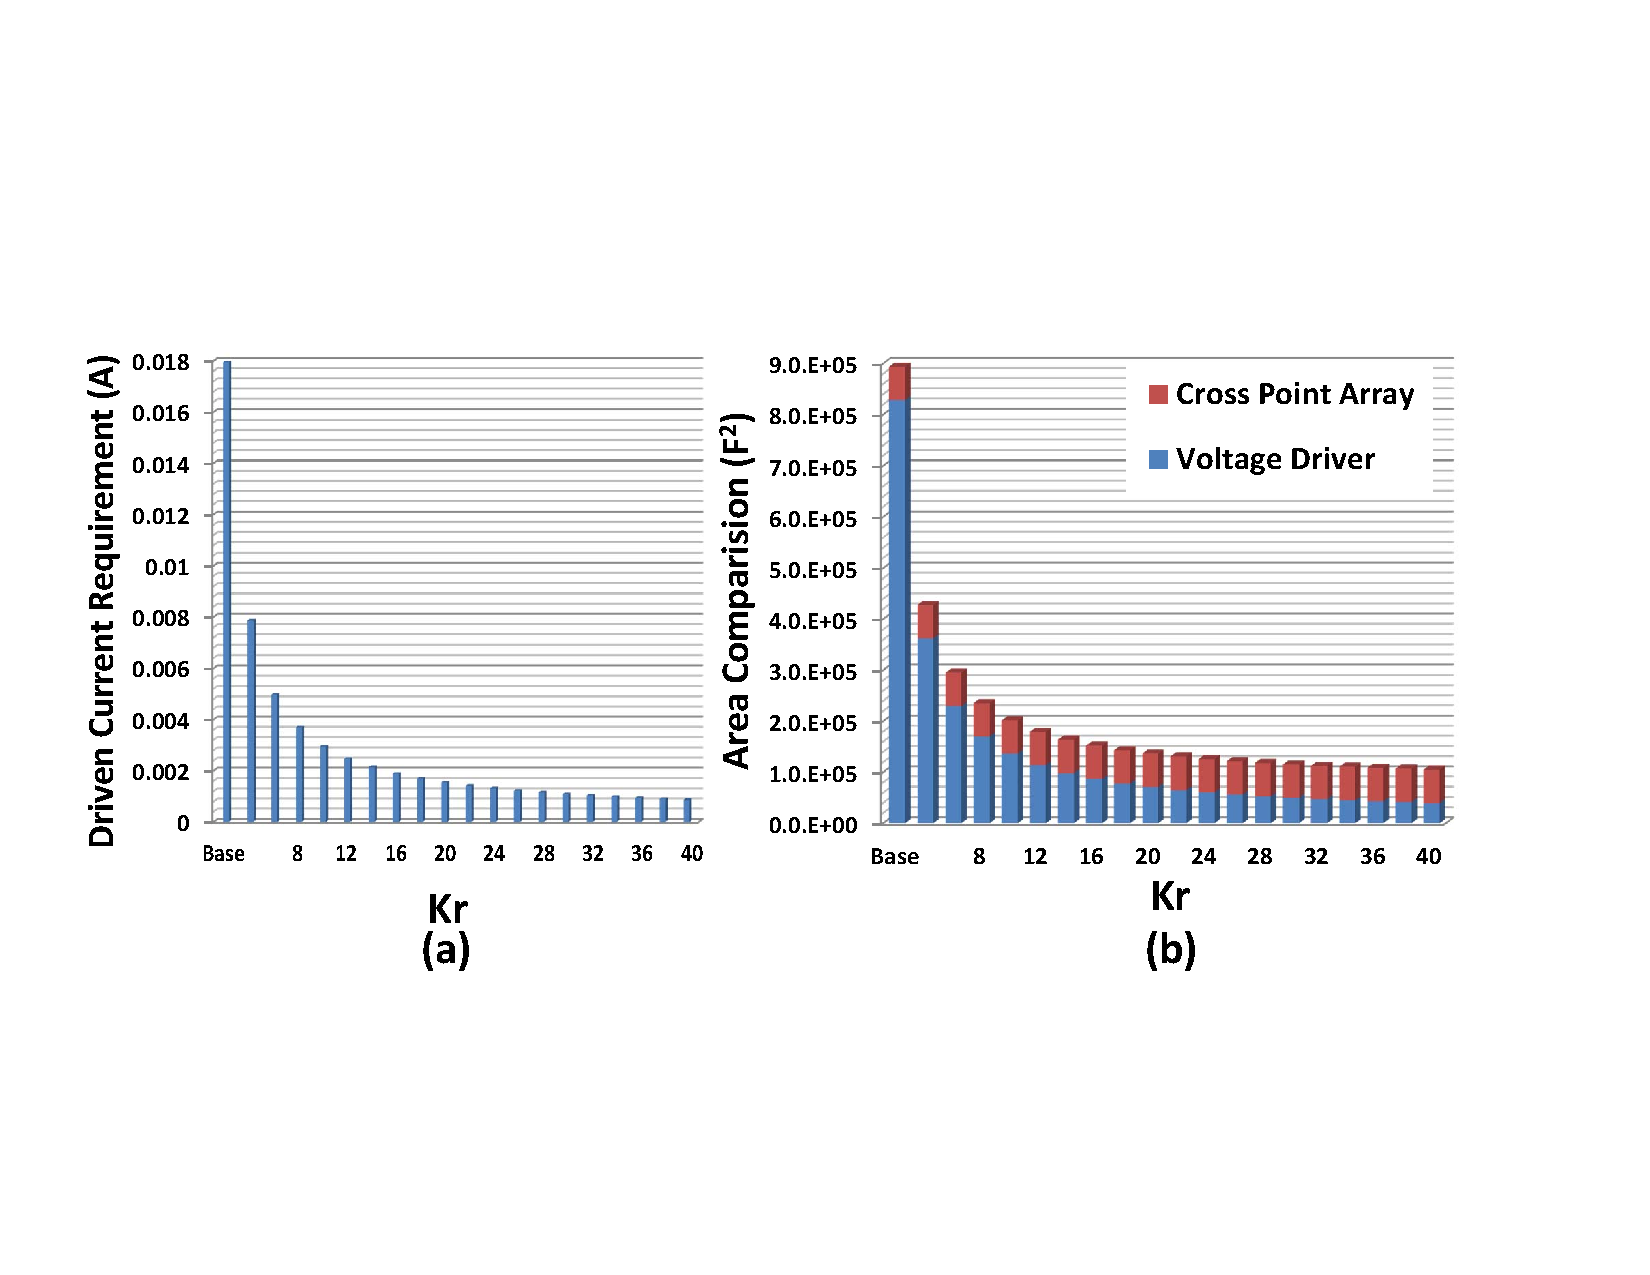
\includegraphics[width=0.5\textwidth]{./figures/area_all.pdf}\\
%  \vspace{-5pt}
%  \caption{The driven current requirements and area overheads with different nonlinearity coefficients}\label{fig:area_all}
% \vspace{-15pt}
%\end{figure}
\begin{figure}[!t]
\centering
  % Requires \usepackage{graphicx}
  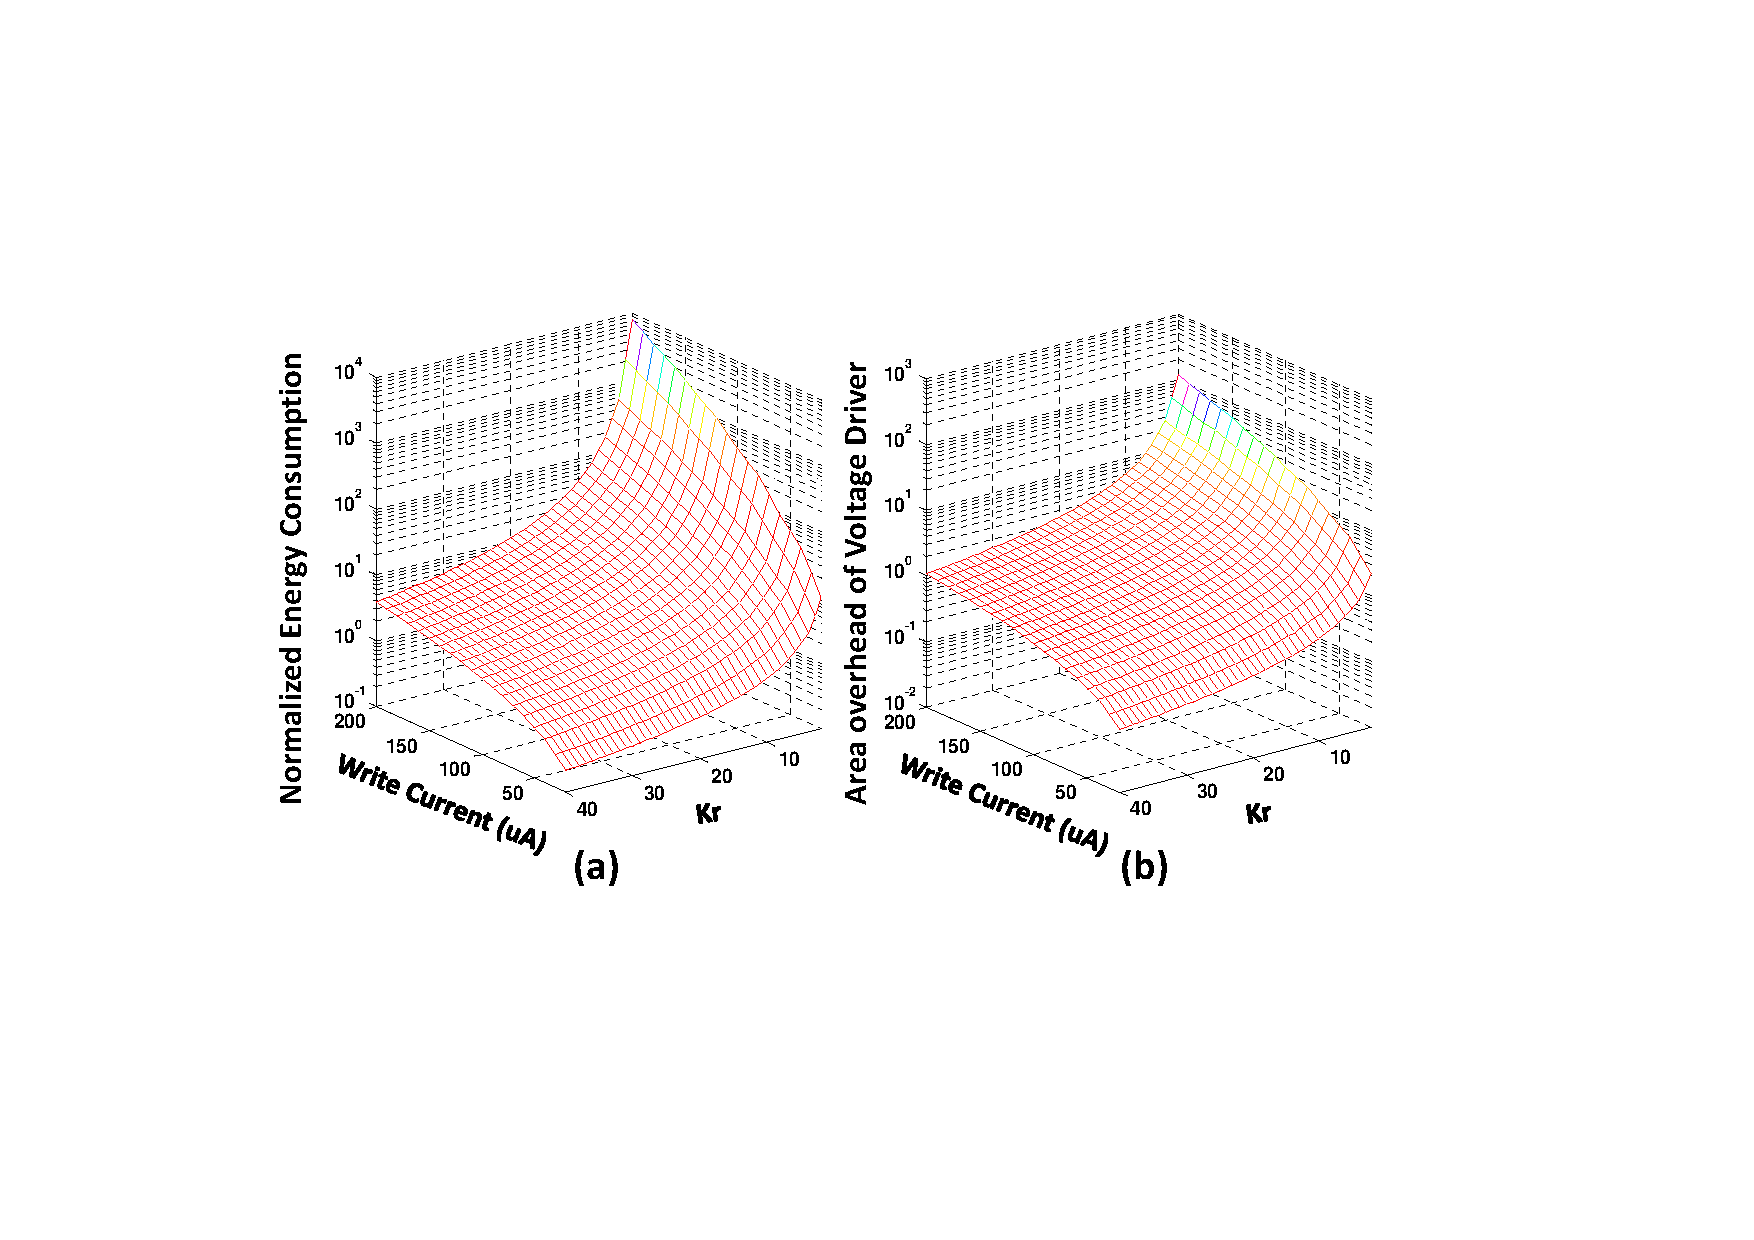
\includegraphics[width=0.5\textwidth]{./figures/E_and_A}\\
\vspace{-5pt}
  \caption{Energy and area overhead comparison. (a) Energy consumption (normalized to baseline). (b) Area overhead of voltage driver (normalized to the area of cross-point array).}\label{fig:E_and_A}
\end{figure}

%\begin{figure}%[!t]
%\centering
%  % Requires \usepackage{graphicx}
%  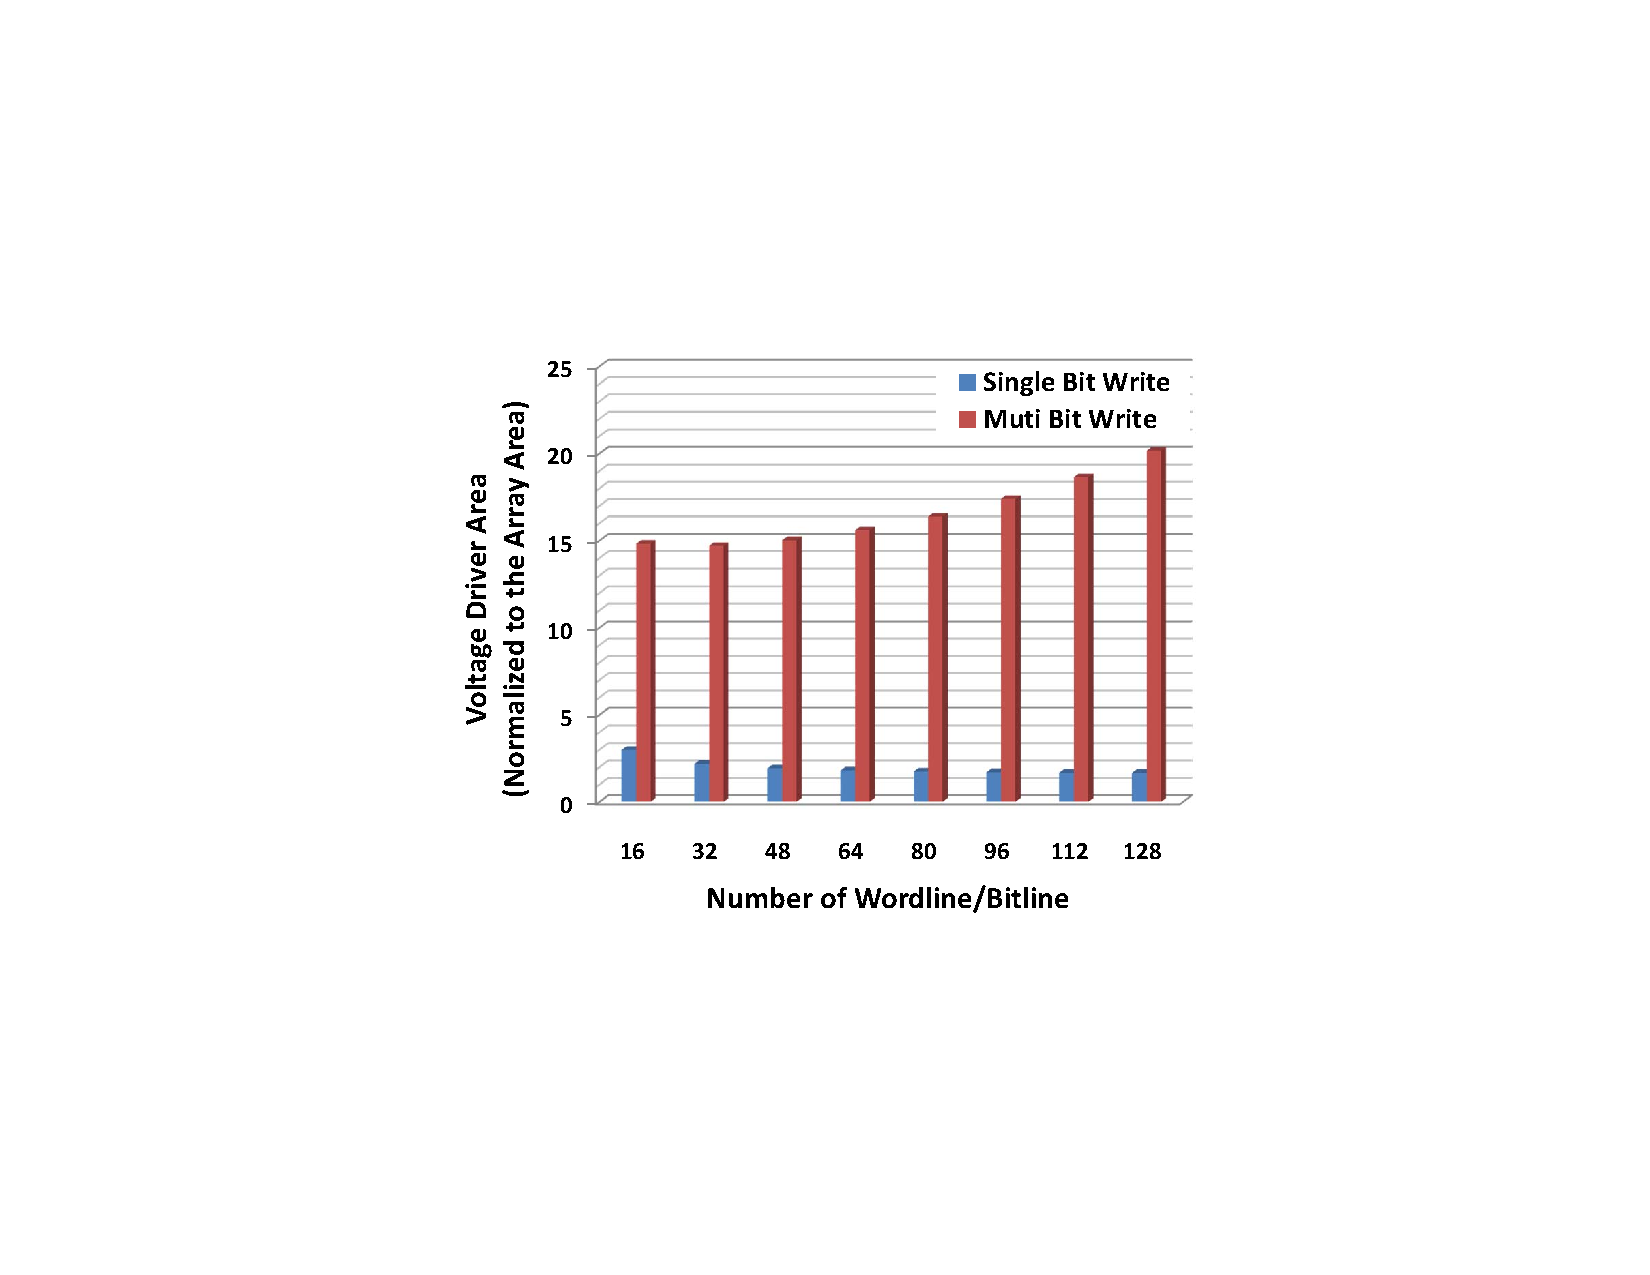
\includegraphics[width=0.35\textwidth]{./figures/Area_kr20_f.pdf}\\
%  \caption{The normalized area overhead of voltage drivers ($K_r=20$, the areas are normalized to the area of cross-point array). }\label{fig:Area_kr20}
%\end{figure}


Different from write operation, the read operation suffers, rather than
benefits, from scaling of nonlinearity or write current. This is simply
because the scaling of nonlinearity and write current will reduce read
current, degrading the read signal ratio. Figure~\ref{fig:sense_margin}(a)
shows the read noise margin with different array size for the baseline
design in Section~\ref{sec:w_and_r}.  As seen, the read noise margin is
reduced at large array size. The impact of nonlinearity and write current
on read noise margin is illustrated in Figure~\ref{fig:sense_margin}(b).
As mentioned, large $K_r$ value and small write current are harmful to the
read noise margin. For example, given a $512 \times 512$, the read noise
margin is less than $10mV$ for $K_r=40$ and $I_w=40\mu A$, which makes it
very difficult to sense the state of the selected memory cell using
traditional sense amplifiers.

%the nonlinearity increases the resistance of half LRS and therefore the
%resistance difference between HRS and LRS cells is reduced; on the other
%hand, .
\begin{figure}[!t]
\centering
  % Requires \usepackage{graphicx}
  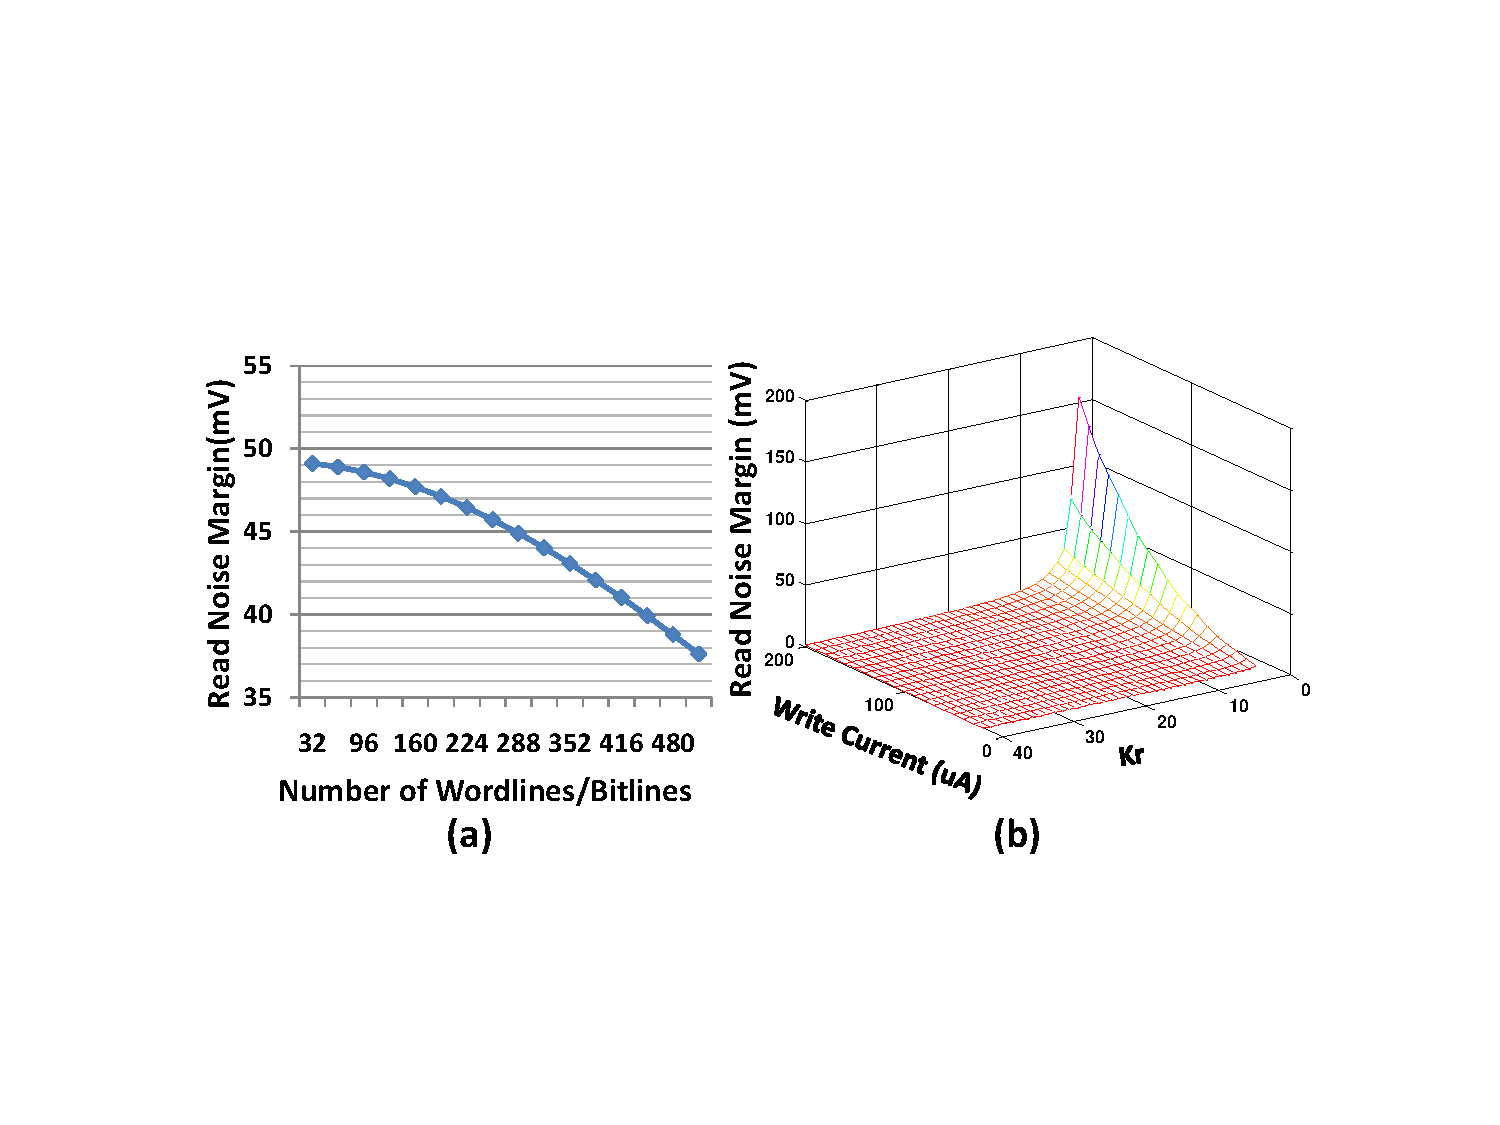
\includegraphics[width=0.5\textwidth]{./figures/read}\\
  \caption{Read noise margin with (a) different array size and (b) scaling of nonlinearity and write current.}\label{fig:sense_margin}
  \vspace{-15pt}
\end{figure}

Therefore, by given the array size and read noise margin constraint, an
"optimal cell" with nonlinearity of $K_{r\_opt}$ and write current of
$I_{on\_opt}$ can be explored. For example, when the array size is fixed
at $512 \times 512$ and the minimum noise margin is $50mV$, a cross-point
array with ReRAM cells, which have $K_{r\_opt} = 9$ and $I_{on\_opt} =
40mA$, is the most energy and area efficient design.


%\subsection{Read Operation}
%In this section we applied the similar sensing scheme as
%\cite{crossbar_TED_2010} and \cite{crossbar_NANO08_Flocke}. In order to
%read cell $R_{i,j}$, the $i^{th}$ wordline is biased at $V_{READ}$ and all
%of the other wordlines and bitlines are grounded. Then the state of the
%selected cell is read out by measuring the voltage across $R_s$. The
%energy consumption for read operation can be analyzed by the same way as
%that of the write operation. Since the read voltage is much smaller than
%write voltage, the read energy is expected at least one order smaller than
%write operation. Additionally, since the read voltage/current is much
%lower than the write, we believe that the voltage drivers can always
%provide enough current for the read operation if they meet the current
%requirement for write operation. Therefore, we can conclude that the area
%overhead of voltage drivers is determined by the write current. However,
%the reliability of read operation is different from the write operation.
%The read reliability is determined by the voltage swing for reading HRS
%and LRS cells. Figure~\ref{fig:sense_margin} (a) shows the voltage swing
%with different array sizes and $K_r$ values. Large array sizes and large
%nonlinearity are harmful to the voltage swing: on the one hand, a larger
%array has more sneak paths, making the output voltage very sensitive to
%the data pattern of unselected cells; on the other hand, the nonlinearity
%increases the resistance of LRS and therefore the resistance difference
%between HRS and LRS cells is reduced. In order to improve the reliability
%of the read operation, a two-step sensing scheme can be applied, which
%senses the current of an unselected cell first, then the overall current
%is sensed, and after that the current difference is converted to the
%output voltage. The voltage swing of this two-step sensing scheme is shown
%in Figure~\ref{fig:sense_margin} (b). By using this two-step sensing
%schemes, the voltage swing for a given array size and nonlinearity
%coefficient is doubled.
%
%
%
%\begin{figure}[!t]
%\centering
%  % Requires \usepackage{graphicx}
%  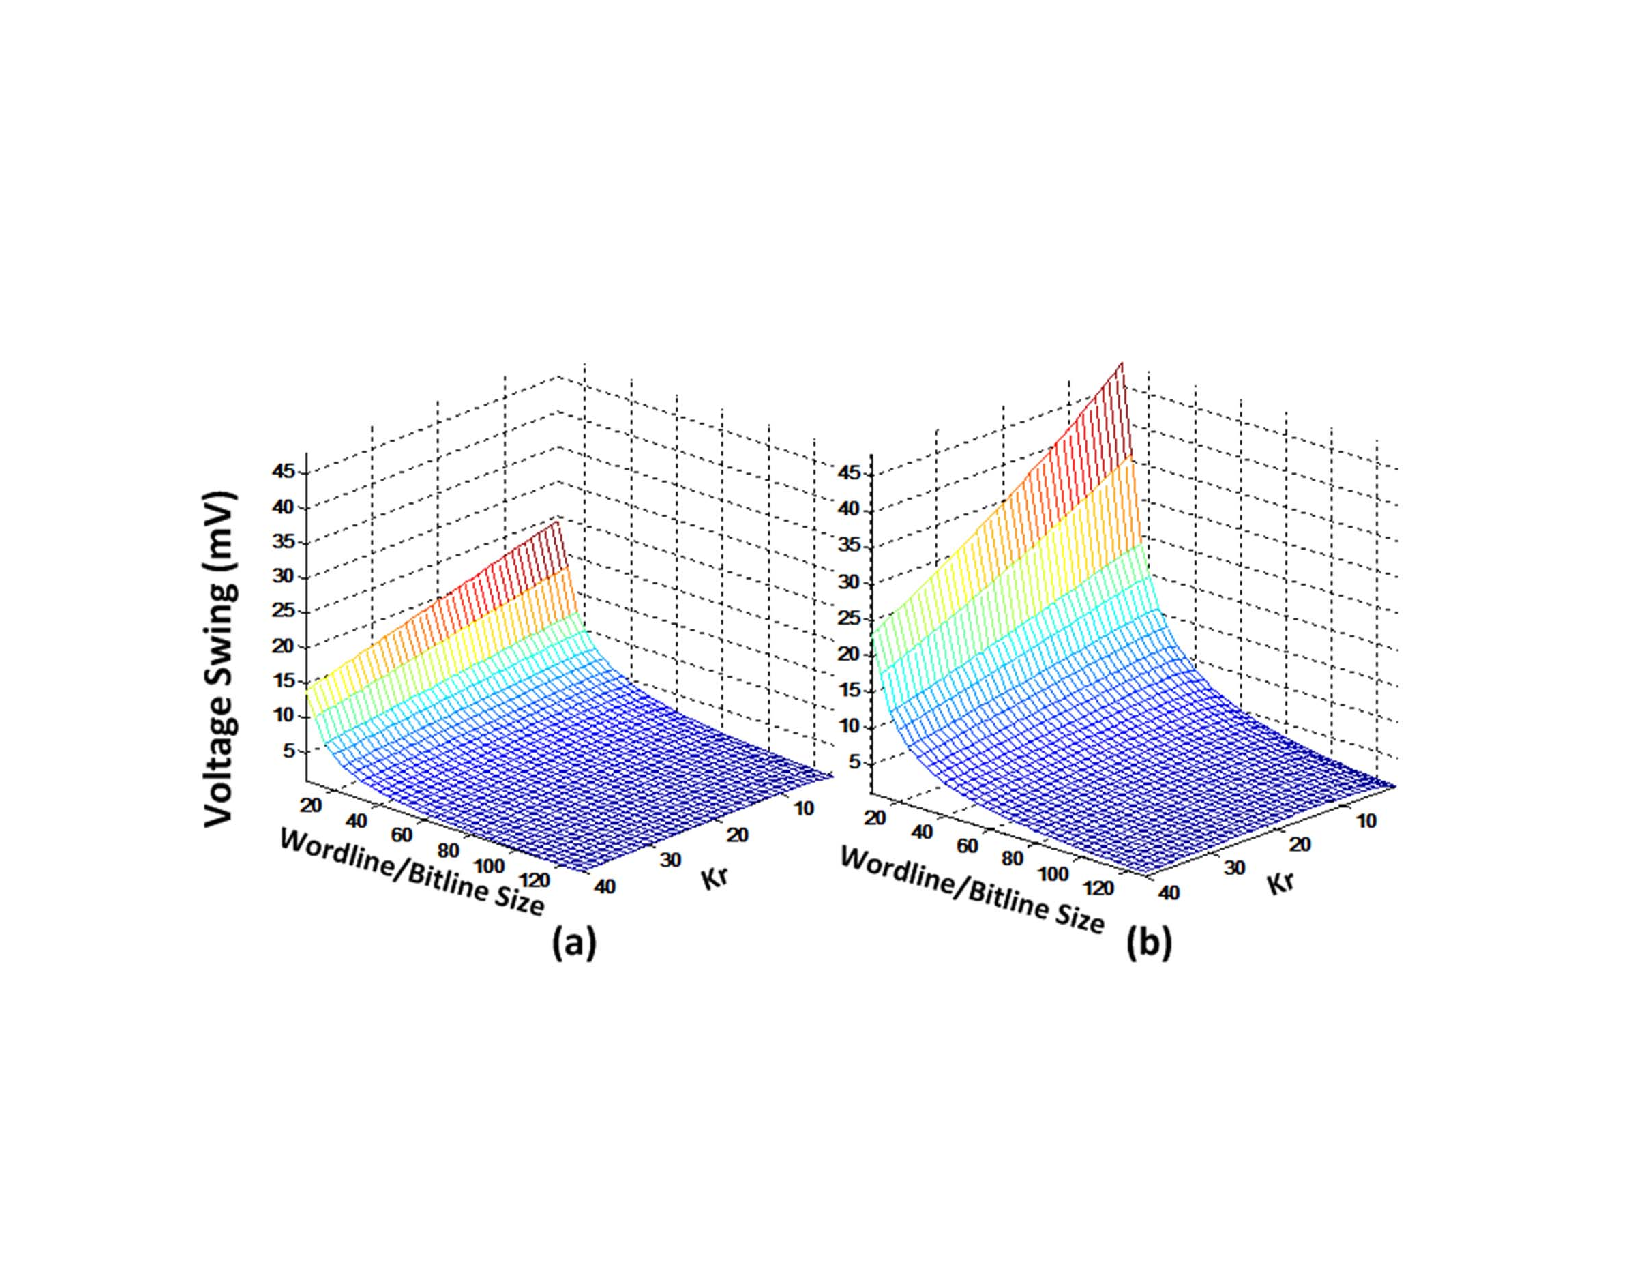
\includegraphics[width=0.5\textwidth]{./figures/sense_margin_f}\\
%  \caption{Relationships among the voltage swing, array size and nonlinearity. (a) Normal sensing scheme; (b) Two-step sensing scheme}\label{fig:sense_margin}
%\end{figure}
